\chapter{Context}

% Introduction of gaming in general and why its worth researching
The focus of this thesis centers on the dynamic landscape of gaming and its ever-evolving environment, which continuously adapts alongside technological progressions and shifting player preferences.\newline

% Introduction of multiplayer games and lag+cpu usage (the problem)
Within this environment, multiplayer experiences stand out as among the most complicated to develop. Unlike single-player or local multiplayer games, where actions are confined to a single system, the complexity escalates with multiple players, amount of events happening in the scene at once, varied network conditions, and the inherent uncertainties of data transmission. In this case two primary challenges emerge: CPU processing (in order to have a large scale games) and network latency (which hinders multiplayer experiences). At the core of this dilemma lies the persistent issue of lag – the delay encountered in transmitting data over the internet, influenced by factors such as geographical distance, network congestion, and computational capabilities which can hinder event the best (in other cases) games \cite{Effects_of_latency}. This latency and computational load can impede players from fully enjoying expansive games, disrupting gameplay flow and diminishing overall enjoyment, underscoring the critical need for effective strategies to mitigate latency especially in combination with games with high CPU usage.\newline

% Introduction of rollback netcode 
Before the first appearance of rollback netcode solutions, online gaming predominantly relied on delay-based systems. These systems aimed for perfect synchronization between players, requiring both parties to wait for each other's inputs before advancing the game to the next frame.\cite{Delaybased_rollback_explanation}.\newline

%correct this one
In contrast, rollback netcode especially in combination with lockstep and player prediction revolutionized online gaming with its approach, addressing the challenges of latency in fast-paced games where reaction windows can be as narrow as 100 milliseconds. Rollback netcode attempts to remedy this with speculative execution: it attempts to predict remote inputs (when latency prevent them to arrive on time) based on prior inputs and roll back and replay the simulation only when necessary. This allows games to continue simulation as if the game were entirely local. Rollback netcode ensures that players experience minimal disruptions (players only notice the network latency if the predictions are wrong), making for a much smoother online experience. \cite{Rollback_overview}\newline

% Introduction of GGPO
At the forefront of this shift was GGPO (Good Game Peace Out), a pioneering networking framework that introduced rollback netcode with lockstep and player prediction in late 2006. The GGPO networking SDK is designed to facilitate the seamless incorporation of rollback networking into both new and existing games. Furthermore, in 2019, the framework transitioned to an MIT license, making it accessible to a wider range of developers. \cite{GGPO_page}\newline

% Introduction of gaming engines
Another crucial aspect of game development is the gaming engine, which serves as the foundation upon which video games are built. Gaming engines provide developers with a comprehensive suite of tools and functionalities to create games efficiently. \cite{Game_engines_comparison}. While some companies develop their own proprietary engines, many developers, especially indie game developers, find it easier to leverage existing solutions.\newline

% Introduction of UNITY
Among the array of gaming engines available, Unity stands out as one of the most prominent and versatile options in the industry. Renowned for its accessibility, Unity offers a robust feature set while remaining free to use until a certain revenue threshold is reached. This accessibility has democratized game development, allowing developers of all levels to create immersive experiences. \newline

% Introduction of DOD
Before delving deeper into the details of game development, it's essential to discuss the concept of Data-Oriented Design (DOD), which addresses a longstanding challenge stemming from the disparity between CPU computation power and memory handling capabilities (as illustrated in Figure \ref{fig:cpu-memory}).

DOD represents an approach to software development that prioritizes the efficient organization and manipulation of data for optimal performance. In contrast to traditional Object-Oriented Design (OOD), which emphasizes encapsulating data and behavior within objects, DOD focuses on structuring data in a manner that maximizes locality and minimizes cache misses. This emphasis on data organization enables developers to leverage modern hardware architectures more effectively, unlocking the full potential of multi-core processors and achieving higher levels of performance and scalability.

The benefits of DOD become particularly evident in performance-critical domains like game development, where achieving high frame rates and responsiveness is utmost important. By aligning data layout with processing requirements and minimizing memory access overhead, DOD enables developers to create more responsive and visually stunning games that fully utilize the capabilities of modern hardware. \cite{DOD_in_games}, \cite{DOD_applications_in_games}\newline

\begin{figure}[h]
    \centering
    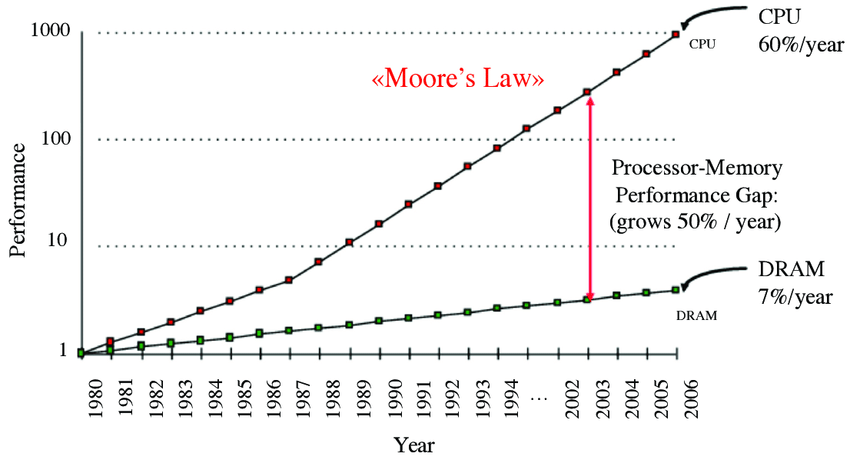
\includegraphics[scale=0.4]{images/CPUvsMEMORY.png}
    \caption{CPU and Memory performance difference over the years [2]}
    \label{fig:cpu-memory}
\end{figure}

% Introduction of DOTS
The Data-Oriented Technology Stack (DOTS) in Unity represents a paradigm shift in game development, leveraging Data-Oriented Design (DOD) principles to maximize performance and scalability. Built upon the Entity-Component-System (ECS) architecture, DOTS decouples data and behavior, enabling developers to optimize hardware utilization and minimize overhead. This approach prioritizes efficient data organization and processing, allowing developers to harness the full potential of modern hardware architectures.\newline

Currently, there is significant potential in merging GGPO and DOTS, leveraging the superior CPU performance of DOTS and the multiplayer rollback netcode solution provided by GGPO.
